% Chương 1

\chapter{TỔNG QUAN VỀ ĐỀ TÀI} 

\label{Chapter1} 

%----------------------------------------------------------------------------------------

% Định nghĩa một số lệnh cần thiết để điều chỉnh định dạng cho một số nội dung nhất định trong bài
\newcommand{\keyword}[1]{\textbf{#1}}
\newcommand{\tabhead}[1]{\textbf{#1}}
\newcommand{\code}[1]{\texttt{#1}}
\newcommand{\file}[1]{\texttt{\bfseries#1}}
\newcommand{\option}[1]{\texttt{\itshape#1}}

%----------------------------------------------------------------------------------------


\section{Khái niệm Học máy (Machine Learning)}

Học máy (Machine learning) là một lĩnh vực của trí tuệ nhân tạo (AI) tập trung vào việc xây dựng các mô hình toán học và thuật toán cho phép máy tính tự động học từ dữ liệu và cải thiện hiệu suất của chúng trong một tác vụ cụ thể. 

\begin{figure}[h!]
	\centering
	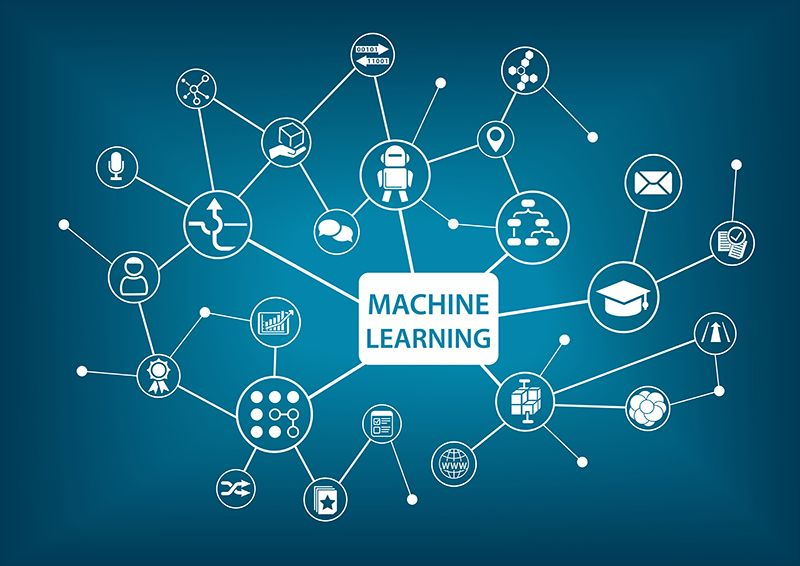
\includegraphics[width=0.65\textwidth]{ML.jpg}
	\caption[Machine Learning.]{Machine Learning.}
	\label{fig:ML}
\end{figure} 

Học máy được sử dụng rộng rãi trong nhiều lĩnh vực như xử lý ngôn ngữ tự nhiên, thị giác máy tính, nhận dạng giọng nói, dự đoán tín dụng và nhiều ứng dụng khác. Các phương pháp học máy phổ biến bao gồm học có giám sát, học không giám sát và học tăng cường.

\section{Tầm quan trọng của Machine Learning}

\begin{itemize}
	\item Học máy đóng vai trò rất quan trọng trong nhiều lĩnh vực bởi vì nó cung cấp cho chúng ta khả năng tự động hóa các tác vụ phức tạp và tối ưu hóa quy trình. 
	
	\item Xử lý các lượng dữ liệu lớn và phân tích chúng để tìm ra các mẫu và thông tin hữu ích.
	
	\item Cho phép dự đoán kết quả và đưa ra quyết định dựa trên tập dữ liệu đã học. Nhờ vào những ứng dụng của nó, học máy đã có ảnh hưởng to lớn đến nhiều lĩnh vực như y tế, tài chính, sản xuất, marketing, và nhiều lĩnh vực khác.
\end{itemize}

\section{Hệ thống nhận diện khẩu trang và cảm xúc}

Tuy dịch bệnh Covid 19 đã dần được đẩy lùi nhưng vẫn có nguy cơ bùng phát trở lại cùng với nhiều biến thể phức tạp. Bên cạnh đó, với sự xuất hiện nhiều loại bệnh lây truyền qua đường hô hấp đã thúc đẩy việc tạo ra những ứng dụng góp phần hỗ trợ việc phòng tránh bệnh, giúp cho người dân dễ dàng kiểm soát việc đeo khẩu trang đúng cách, giảm thiểu nguy cơ lây lan dịch bệnh trên diện rộng.

Việc áp dụng công nghệ Deep Learning vào bài toán nhận diện cảm xúc khuôn mặt và việc có hay không đeo khẩu trang đang được dự án triển khai và phát triển. Ứng dụng mô hình mạng nơ-ron tích chập (Convolutional Neural Network – CNN) được sử dụng rất nhiều trong lĩnh vực dự đoán hình ảnh. Trong báo cáo này, nhóm xây dựng một mô hình học máy sử dụng mô hình mạng tích chập CNN để nhận diện việc có hay không đeo khẩu trang cũng như kết hợp xây dựng mô hình nhận diện cảm xúc.

\section{Tổng quan bài toán} 

\subsection{Mô tả bài toán thực tế} 

\begin{itemize}
	\item Sử dụng mạng nơ-ron tích chập (CNN) huấn luyện một mô hình có thể nhận biết : Người có đeo khẩu trang , Không đeo khẩu trang và Đeo sai cách.
	
	\item Nếu không đeo khẩu trang thì có thể nhận biết cảm xúc cũng dùng mạng nơ-ron tích chập (CNN) để huấn luyện mô hình nhận dạng cảm xúc.
	
	\item Hệ thống camera để hiển thị lên màn hình trạng thái của việc đeo khẩu trang và cảm xúc.
\end{itemize}

\subsection{Mô tả bài toán chi tiết}

CNN hoạt động bằng cách sử dụng các bộ lọc (filters) để thực hiện phép tích chập (convolution) trên hình ảnh đầu vào. Bộ lọc này sẽ di chuyển trên toàn bộ hình ảnh, tìm kiếm các đặc trưng của hình ảnh bằng cách so sánh các khu vực nhỏ của hình ảnh với một mẫu được học trước. Các đặc trưng được tìm thấy sau đó sẽ được đưa vào một hoặc nhiều lớp ẩn để xử lý và trích xuất thông tin từ các đặc trưng này.

\begin{figure}[h!]
	\centering
	
\includegraphics[width=0.7\textwidth]{anh1.png}
	\caption[Quy trình huấn luyện ]{Quy trình huấn luyện}
	\label{fig:mohinh}
\end{figure} 

Sau khi thông tin được trích xuất, CNN sử dụng một số lớp Fully Connected (FC) để xử lý dữ liệu và cuối cùng đưa ra kết quả dự đoán về việc đeo có đeo khẩu trang không, đeo khẩu trang có đúng hay không.

Việc xây dựng một mô hình CNN cho chẩn đoán đeo khẩu trang yêu cầu một tập dữ liệu lớn về hình ảnh khuôn mặt, trong đó phải có đầy đủ các trường hợp đeo khẩu trang, không đeo khẩu trang, đeo khẩu trang sai cách cùng với tập ảnh về cảm xúc (angry, happy, neutral, fear, disgust,...). Sau đó, mô hình sẽ được huấn luyện trên tập dữ liệu này để học cách phân biệt các đặc trưng của hình ảnh đeo khẩu trang cũng như không đeo và đeo sai cách và cảm xúc khuôn mặt.


